\section{Background}
% why is the problem I'm working on interesting?

% figure with number of artifacts & early stop codons found in real data?
%   similar to Reed's figure but create my own, maybe ask for scripts/ideas.

% information age?
Advancements in sequencing technology and the increasing affordability of new
equipment has generated an overflow of genomic information.
The abundance of data being processed today is orders of magnitude greater than
two decades ago. %\green{with no slow down in sigh}.
% As a result, computational tools are required to keep up to properly handle
% large projects.
Unfortunately, the available deluge of genomic data is not free of artifacts.
Uncorrected errors in genomic datasets can lead to erroneous results in
functional and comparative genomic studies \parencite{estimates_schneider_2009}.
This requires requires costly curation practices that discard large amounts of
information.

Sequence alignment is considered a fundamental task in bioinformatics and a
cornerstone step in comparative and functional genomic studies
\parencite{sequence_alignment_rosenberg_2009}.
% An alignment is a hypothesis of which characters from two or more sequences are
% homologous \parencite{problems_cartwright_2009}.
% Inference of homology is an inherently difficult problem since the objective is
% backtracking unique and unobservable historical events
% \parencite{sequence_aln_morrison_2010}.
Sequence alignment is also essential to other analyses, including the
identification of conserved motifs, estimation of evolutionary divergence
between sequences, inference of phylogenetic relationships
\parencite{MSA_kumar_2007}, identification of disease-associated mutations,
measurement of selection, among others
\parencite{sequence_alignment_rosenberg_2009}.

% about programs still not fully addressing sequence homology
Modern sequence analysis began with the heuristic homology algorithms of
Needleman and Wunsch in 1970 \parencite{identification_smith_1981} and has
progressed to arrive at current aligners such as BAli-Phy \parencite{suchard_baliphy_2006},
CLUSTAL$\Omega$ \parencite{clustal_omega_sievers_2011}, MAFFT \parencite{mafft_katoh_2002},
MACSE \parencite{ranwez_macse_2011}, PRANK \parencite{prank_loytynoja_2014}.
However, the alignment of molecular sequences is, in practice, often seen as a
tool and the alignment inference as an ad hoc problem
\parencite{morrison_MSA_2018}.

% what current aligners are missing
A common strategy is to align sequences is a three step approach that (1)
translates DNA sequences to amino acids, (2) performs alignment inference
in the amino acid spaces, to finally (3) back-translate to DNA
\parencite{bininda2005transalign, abascal2010translatorx}.
While this approach is an improvement over DNA models, it discards information,
fails in the presence of artifacts, and has been shown to underperform compared
to alignment at the codon level.
Although some aligners incorporate codon substitution models (e.g. BAli-Phy,
PRANK), they do not support frameshifts or lack a statistical model.
While indels are rarely modeled to appear within codons, it has been estimated
that this is often the case \parencite{indel_phases_zhu_2019}.
When gaps are only considered to appear between codons, the optimal alignment
can be missed (Fig. \ref{fig:indels})

\begin{figure}[h!]
% \begin{framed}
  \begin{minipage}[c]{0.6\textwidth}
    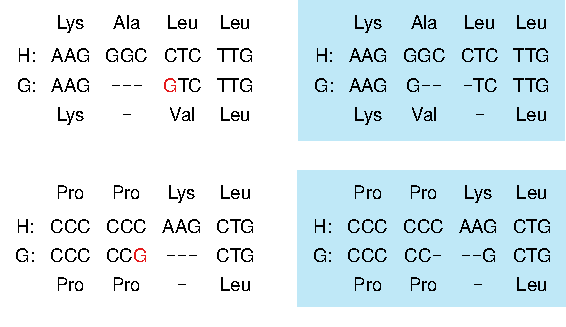
\includegraphics[scale=1]{fig-aln.pdf}
  \end{minipage}\hfill
  \begin{minipage}[c]{0.4\textwidth}
	\caption{Standard algorithms produce suboptimal alignments.
		Rows show possible alignments of gorilla (G) against human (H) sequences.
		The best alignment is highlighted in blue, and nucleotide mismatches are highlighted in red.
		Because standard algorithms do not support within codon indels, they miss the best
		alignment and inflate estimates of sequence divergence.}
	\label{fig:indels}
  \end{minipage}
% \end{framed}
\end{figure}

% Current methods are not able to keep up with the amount of information
% generated.
Frameshifts are common in coding-sequence datasets.
However, these are expected to be errors due to strong purifying selection.
Identifying canonical coding sequences to patch this issue is the most
accessible solution and yet often unsuccessful.
Improving the annotation quality or re-sequencing with higher quality involves
high costs with little reward.
Therefore, researchers are ill-equipped to deal with uncurated heterogeneous
datasets.
To address this need, I propose to develop COATi, a tool that will be able to
generate sequence alignments while correcting for artifacts in a feature-rich
and user-friendly software package.

% Designing a new aligner is not enough if researchers are left alone to infer
% biologically meaningful parameters for COATi's model.
% Therefore, this aligner will be capable of deriving parameter estimates from
% data for an accurate result.
% \green{Expand?}
